\documentclass{article}
\usepackage{titlepage}
\usepackage{geometry}
\geometry{
 a4paper,
 total={170mm,257mm},
 left=10mm,
 right=10mm,
 top=20mm,
 }

\graphicspath{{image/}}

\title{Assembleur et RTN concret}
\subtitle{TP2}
\dateremise{le 19 octobre 2017}
\author{Julien Legault, 1847125}{Billy Bouchard, 1850477}{Groupe B1}%{Nom4, matricule}
\prof{Abdellatif Amrani}


\begin{document}
\maketitle
\section*{Exercice 1}
\subsection*{Recherche d'instruction}
\begin{tabular}{ | l *{17}{|c}|}
	\hline
	\textbf{RTN concret}  & 15 & 14 & 13 & 12 & 11 & 10 & 9 & 8 & 7 & 6 & 5 & 4 & 3 & 2 & 1 & 0 & \textbf{hexa} \\ \hline \hline
	\verb|MA <- PC;|      & 0  & 0  & 1  & 1  & 0  & 0  & 0 & 0 & 0 & 1 & 1 & 0 & 0 & 0 & 0 & 0 & 0x3060        \\ \hline
	\verb|MD <- M[MA] : | & 0  & 1  & 1  & 0  & 1  & 1  & 0 & 0 & 1 & 1 & 0 & 0 & 0 & 0 & 0 & 0 & 0x6CC0        \\
	\verb|PC <- PC + 4; | &    &    &    &    &    &    &   &   &   &   &   &   &   &   &   &   &               \\ \hline
	\verb|IR <- MD|       & 1  & 0  & 0  & 0  & 0  & 0  & 1 & 0 & 0 & 1 & 1 & 0 & 0 & 0 & 0 & 0 & 0x8260        \\ \hline
\end{tabular}

\subsection*{Execution d'une instruction G\'en\'erique}
\begin{tabular}{ | l *{17}{|c}|}
	\hline
	\textbf{RTN concret}        & 15 & 14 & 13 & 12 & 11 & 10 & 9 & 8 & 7 & 6 & 5 & 4 & 3 & 2 & 1 & 0 & \textbf{hexa} \\ \hline \hline
	\verb|A <- R[rc];|          & 0  & 0  & 0  & 0  & 0  & 0  & 0 & 0 & 0 & 1 & 1 & 0 & 1 & 1 & 1 & 0 & 0x006E        \\ \hline
	\verb|MA <- A + IR<11..0>;| & 0  & 0  & 0  & 1  & 0  & 0  & 0 & 0 & 0 & 0 & 1 & 0 & 0 & 0 & 0 & 1 & 0x1021        \\ \hline
	\verb|MD <- M[MA]:|         & 0  & 0  & 0  & 0  & 1  & 1  & 0 & 0 & 1 & 1 & 1 & 0 & 1 & 0 & 1 & 0 & 0x0CEA        \\
	\verb|A <- R[rb];|          &    &    &    &    &    &    &   &   &   &   &   &   &   &   &   &   &               \\ \hline
	\verb|R[ra] <- A oper MD;|  & 1  & 0  & 0  & 0  & 0  & 0  & 1 & 0 & 0 & 0 & 0 & 1 & 0 & 0 & 0 & 0 & 0x8210        \\ \hline
\end{tabular}

\newpage
\subsection*{Simulation}
\begin{figure}[!ht]
	\centering
	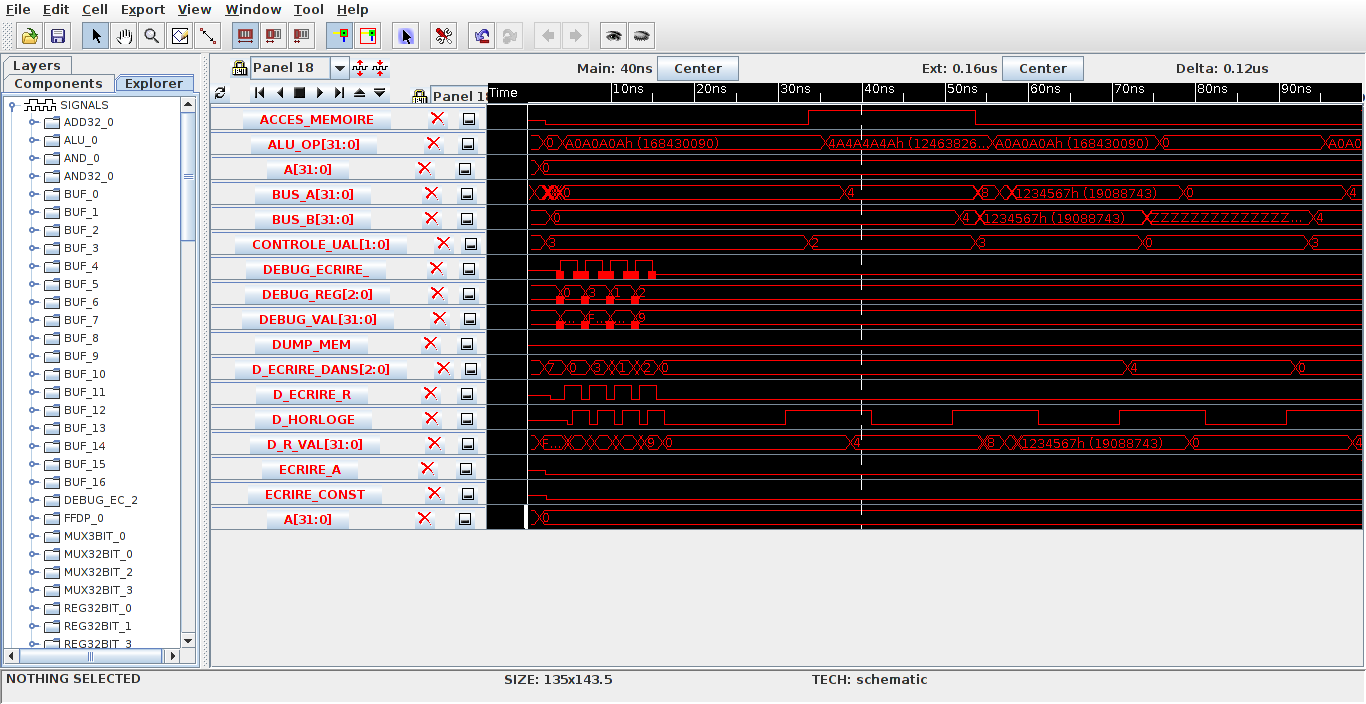
\includegraphics[width=1\textwidth]{e1-q3-p3.png}
	\caption{jusqu'\`a 0.09 us}
	\label{}
\end{figure}
\begin{figure}[!hb]
	\centering
	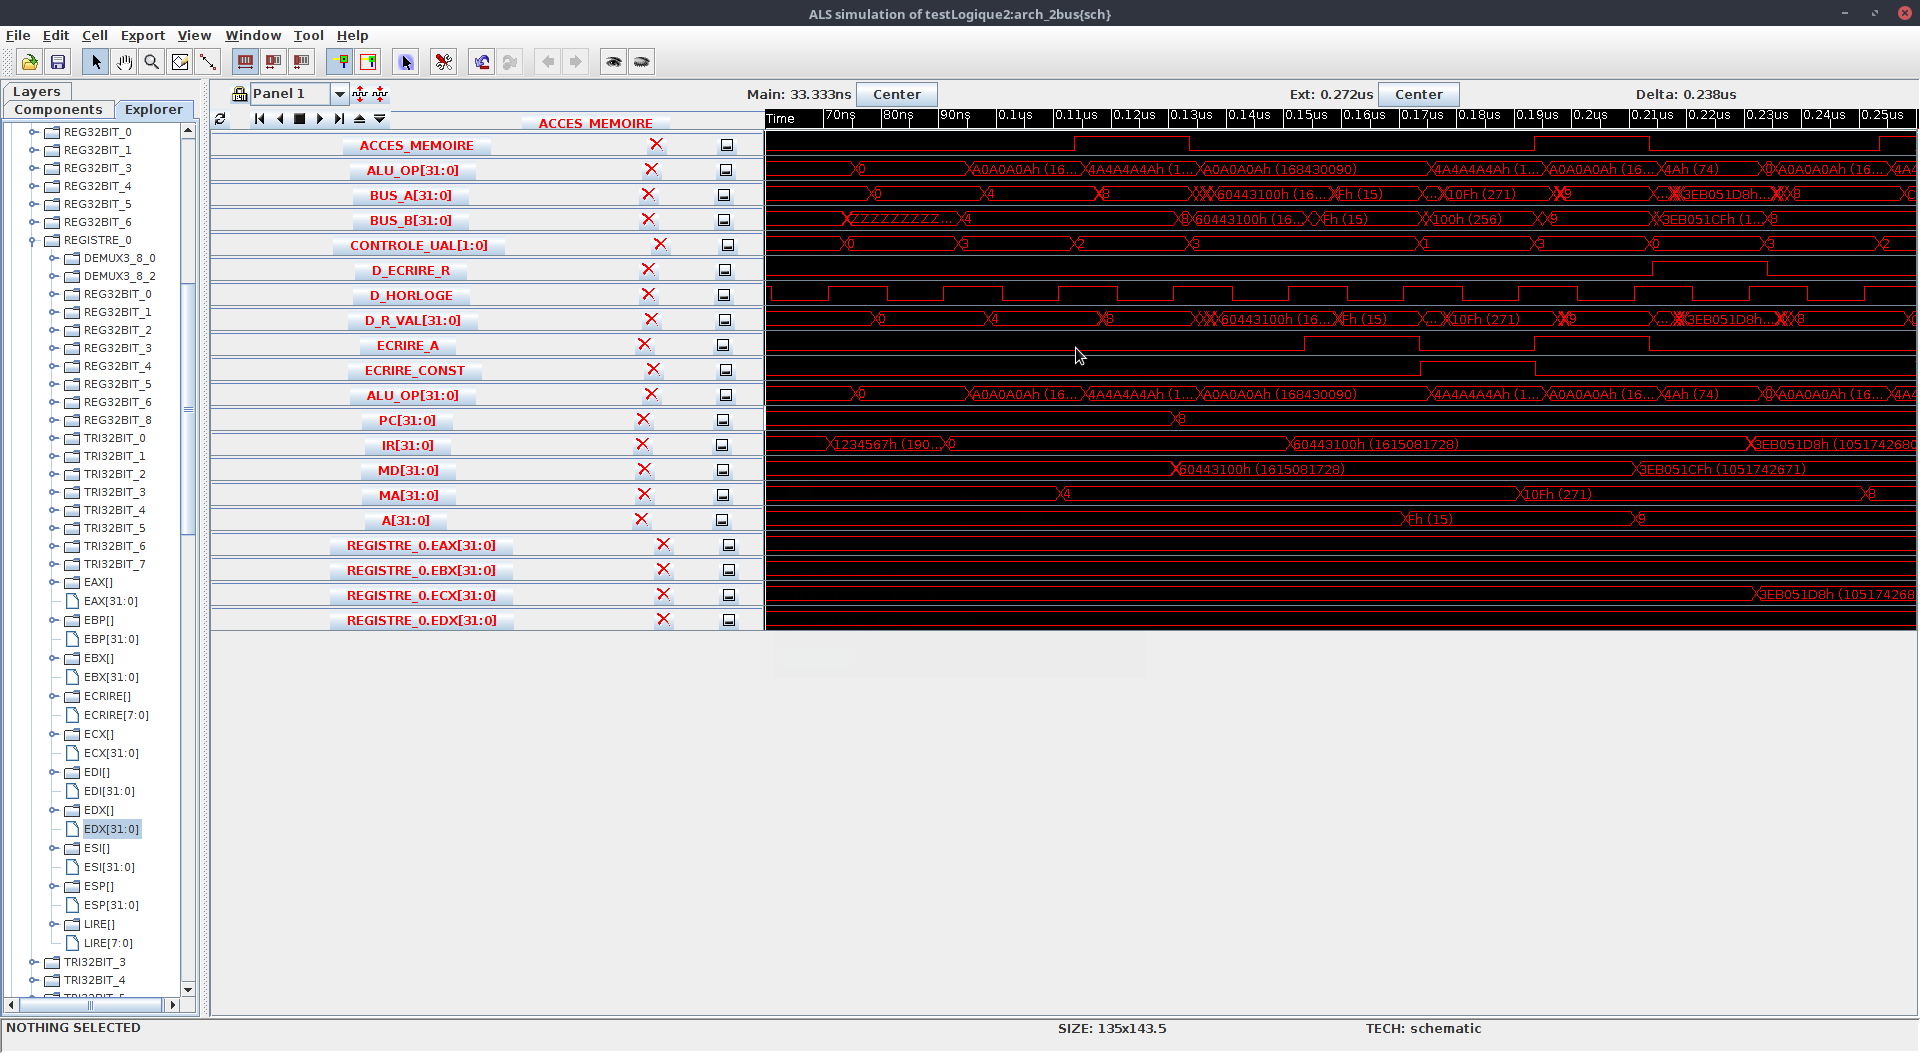
\includegraphics[width=1\textwidth]{e1-q3-p1.png}
	\caption{\`a partir de 0.09 us (curseur en place)}
	\label{}
\end{figure}

\newpage
\subsection*{l'operation NAND}
La valeur a donner est : 0b0000111
on peut le decomposer de cette facon : \\
\verb|op[0:3] = 0111 il s'agit du test logique NAND de la table de veriter | \\
\verb|op[4] = 0 multiplexeur choisi la branche des test logique | \\
\verb|op[5] = 0 addition avec aucune retenue| \\
\verb|op[6] = 0 on ne donne pas la variable a a l'additionneur, on donne 0000| \\
\begin{figure}[!h]
	\centering
	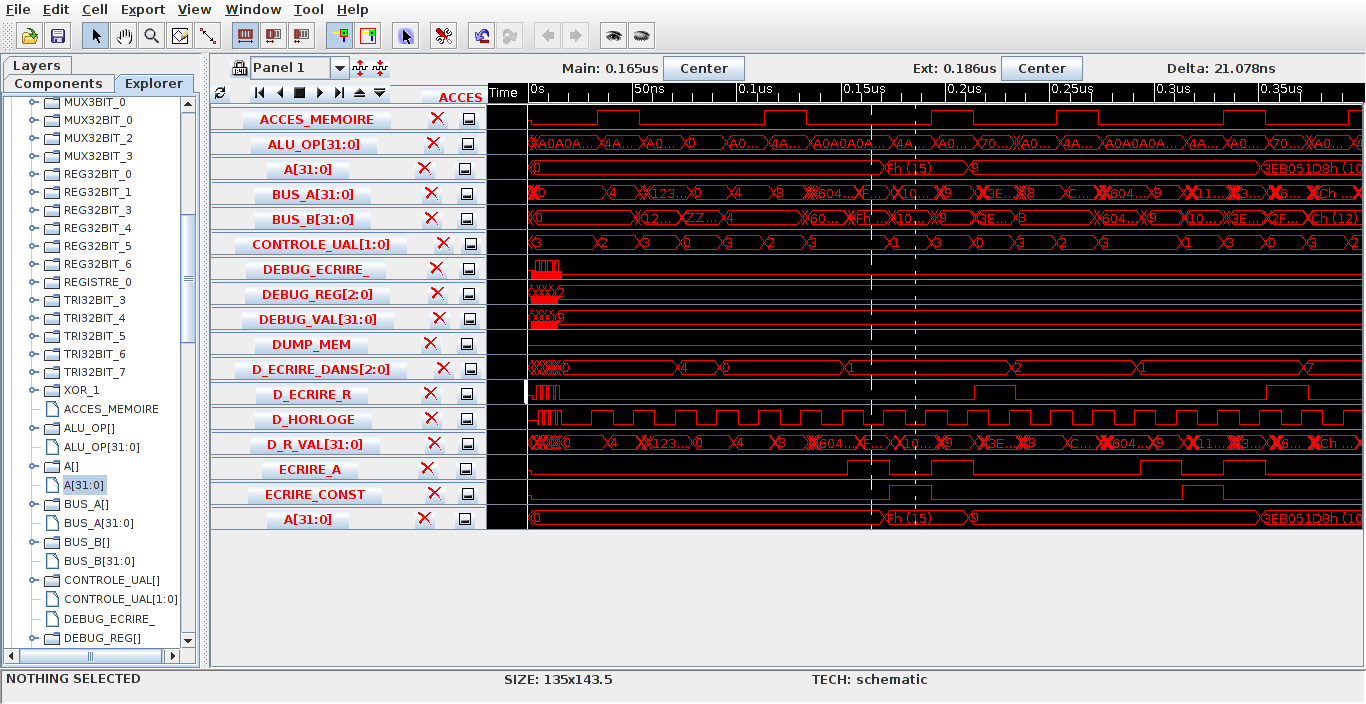
\includegraphics[width=0.85\textwidth]{e1-q4-p1.png}
	\caption{Zoom out pour le NAND}
	\label{}
\end{figure}
\begin{figure}[!h]
	\centering
	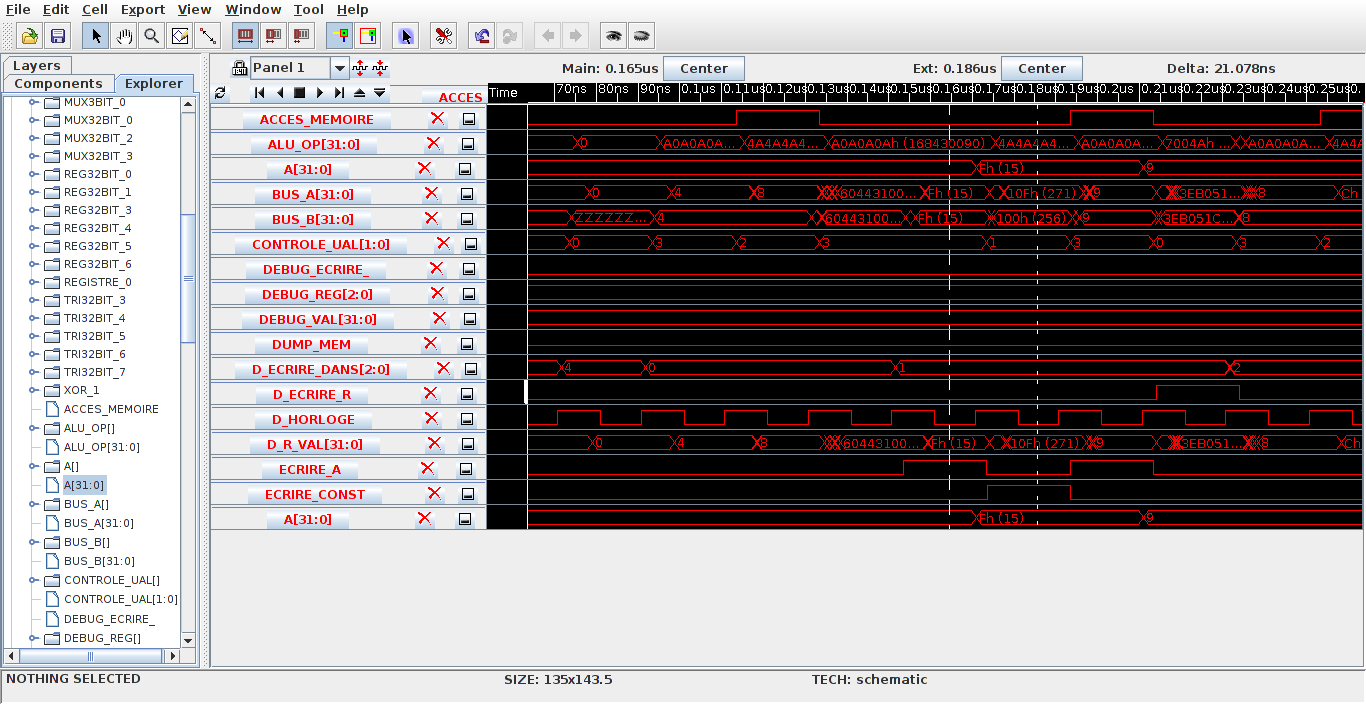
\includegraphics[width=0.85\textwidth]{e1-q4-p2.png}
	\caption{Zoom in pour le NAND}
	\label{}
\end{figure}
\newpage
\subsection*{Compr\'ehension}
\begin{enumerate}[label = (\alph*)]
	\item les deux derniers octets repr\'esentent respectivement la valeur de la constante
            ainsi qu'une partie du registre rc. Si nous observons l'instruction en question, soit
            0x05 0x55 0x55 0x55, nous voyons que l'opcode soit les 5 bits les plus significatifs sont 00000. 
             Comme l'opcode est 0, l'instruction devra être un NOP, soit prendre uniquement l'opération indiqué 
             dans le reste des bits de l'instruction. Un opcode effectuant la même opération pourrait être 0x7654321.
             du coup l'opcode vaut 0 et aucune opération ne sera forcé.
	
	\item On peut utiliser un des bus pour acheminer de l'information
	      alors que l'on fais une autre chose avec l'autre bus
	      Nous l'avons utilis\'ee lorsque nous faisions les calculs en amenant une variable
	      sur le bus B et en sortant la valeur de retour sur le bus A.
	\item Oui c'est plus flexible car nous pouvons combiner plusieurs
	      op\'eration dans une seule ligne d\^u \`a la grande libert\'e du second bus.
\end{enumerate}

\end{document}
